\section{Model Architecture and Rationale}

The model architecture employed in this project is a hybrid Autoencoder-LSTM, combining the strengths of autoencoders for dimensionality reduction and LSTMs for temporal modeling. This architecture is particularly well-suited for the problem of house price prediction due to the high-dimensional and time-series nature of the dataset.

\subsection{High Dimensionality of Data and the Role of Autoencoders}

The dataset incorporates numerous economic indicators, such as the MLS Home Price Index (HPI), Consumer Price Index (CPI), and Canada Prime Rate, along with their revisions and interpolations. These variables, when combined with data resampled at daily intervals, result in a high-dimensional feature space. High-dimensional data can lead to challenges such as increased computational costs, redundancy among features, and overfitting.

To address these issues, an autoencoder is used as the initial component of the model. The autoencoder includes:

\begin{figure}[H]
    \centering
    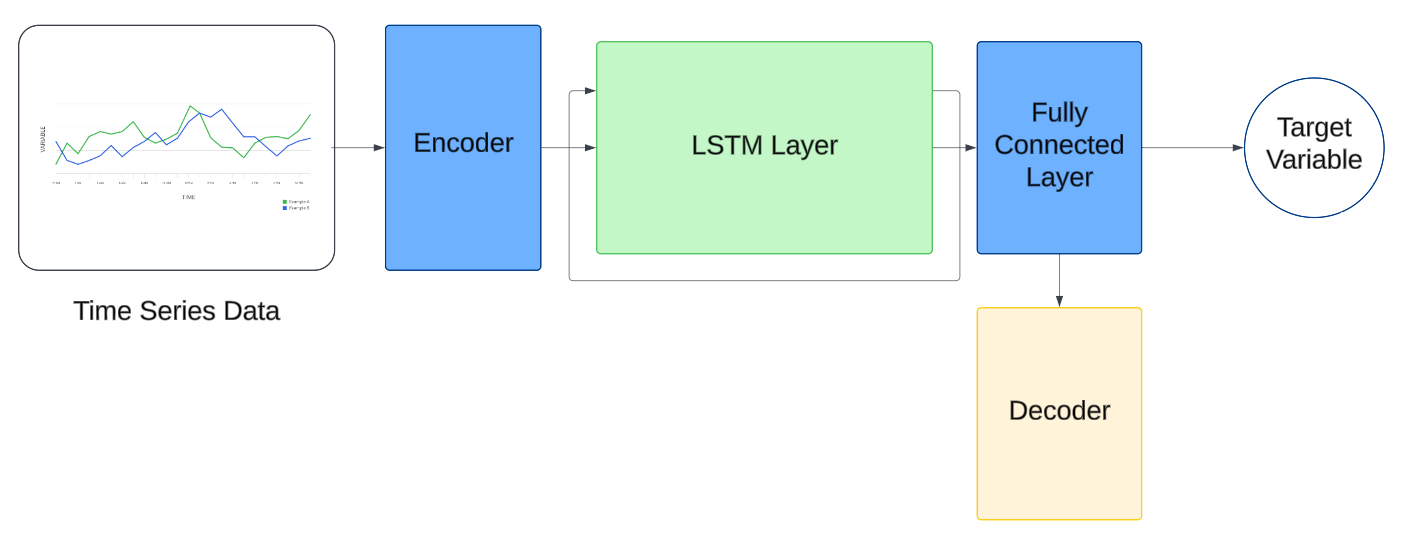
\includegraphics[width=0.8\textwidth]{images/architecture.png}
    \caption{Hybrid Autoencoder-LSTM Model Architecture}
    \label{fig:architecture}
\end{figure}

\begin{itemize}
    \item \textbf{Encoder Layer:} Reduces the input dimensionality by compressing the features into a latent space representation, retaining only the most informative features. This helps eliminate redundant and less relevant information while mitigating the risk of overfitting.
    \item \textbf{Decoder Layer:} Optionally reconstructs the original input from the latent space, enabling auxiliary supervision during training. This reconstruction step ensures the encoder captures the essential structure of the input data.
\end{itemize}

By using an autoencoder, the model focuses on the core features that influence house prices, reducing noise and improving computational efficiency.

\subsection{Time-Series Nature of Data and the Role of LSTMs}

The dataset is inherently sequential, as it includes daily observations of economic indicators. Predicting house prices depends not only on the current values of these indicators but also on their historical patterns and trends. Long Short-Term Memory (LSTM) networks are ideal for such tasks because they:

\begin{itemize}
    \item \textbf{Capture Temporal Dependencies:} LSTMs use gates to selectively remember or forget information from previous time steps, making them effective in identifying trends and temporal relationships in the data.
    \item \textbf{Avoid Vanishing Gradients:} Unlike traditional RNNs, LSTMs are designed to retain information over long sequences without suffering from vanishing gradient issues, enabling them to model long-term dependencies effectively.
\end{itemize}

In this architecture, the compressed latent representation from the autoencoder is fed into the LSTM layers. This combination ensures that the model operates efficiently in high-dimensional spaces while accurately capturing the sequential nature of the data.

\subsection{Advantages of Combining Autoencoders and LSTMs}

The hybrid Autoencoder-LSTM architecture leverages the strengths of both components:

\begin{itemize}
    \item The autoencoder ensures dimensionality reduction, noise elimination, and focus on core patterns, which is essential given the high-dimensional input data.
    \item The LSTM effectively models the temporal dependencies in the reduced feature space, improving the model’s ability to predict trends over time.
\end{itemize}

The combination reduces computational complexity and enhances the robustness and accuracy of predictions by tackling both high-dimensionality and sequential modeling challenges.